\documentclass[11pt,a4paper]{article}
\usepackage[utf8]{inputenc}
\usepackage[T1]{fontenc}
\usepackage{amsfonts}
\usepackage[french]{babel}
\frenchbsetup{StandardLists=true} % à inclure si on utilise \usepackage[francais]{babel}
\usepackage{enumitem}
\usepackage{amssymb}
\usepackage{amsmath}
\usepackage[left=2cm,right=2cm,top=2cm,bottom=2cm]{geometry}
\usepackage{multirow}
\usepackage[dvipsnames]{xcolor}

\usepackage[T1]{fontenc}
\usepackage{fouriernc}
\usepackage{graphicx}

\usepackage{setspace}
\singlespacing

\usepackage{pstricks}
\usepackage{xkeyval}
\usepackage{pst-labo}


\usepackage{multicol}
\usepackage{caption}
\usepackage{fancyhdr}
\pagestyle{fancy}
\renewcommand\headrulewidth{1pt}
\fancyhead[L]{Lycée Denis Diderot }
\fancyhead[R]{Classe de 1 Bac Pro }
\setcounter{page}{6}\fancyfoot[C]{page \thepage}
\fancyfoot[R]{Année 2024-2025}
\fancyfoot[L]{Alexis RUIZ}
\usepackage{multirow,tabularx,booktabs}
\usepackage[tikz]{bclogo} 

\newcommand{\cadreblanc}[1]{%
\medskip\framebox[\linewidth][c]{%
\rule{0mm}{#1mm}}\par
\medskip}

\usepackage{awesomebox}
\setlength{\aweboxvskip}{0mm}
\usepackage{pifont}
\usepackage{chemmacros}
\chemsetup{modules=all}
\setlength{\columnseprule}{.25mm}

\renewcommand{\arraystretch}{2}
\newcommand*\acocher{\quitvmode{\fboxsep0pt \fboxrule0.8pt \fbox{\vrule height1.8ex depth.1ex width0pt \vrule height0pt depth0pt width1.9ex }}}

\newcolumntype{C}[1]{>{\centering\arraybackslash }b{#1}}

\newcommand{\code}{\awesomebox[black]{2pt}{

\includegraphics[scale=0.15]{images/frame.png}
}{black}}

\newcommand{\moteur}{\awesomebox[black]{2pt}{

\includegraphics[scale=1]{images/moteur.jpg} 
}{black}}

\newcommand{\defbox}{\awesomebox[black]{2pt}{
\includegraphics[scale=0.5]{images/appel exam.png}}{black}}

\newcommand{\defconclusion}{\awesomebox[black]{2pt}{\rotatebox{90}{\Large{\textbf{Conclusion}}}}{black}}

  \newenvironment{itemize*}%  % listes compactes
    {\begin{itemize}%
      \setlength{\itemsep}{0pt}%
      \setlength{\parskip}{0pt}}%
    {\end{itemize}}

\frenchbsetup{StandardLists=true}



\begin{document}

\flushleft \textbf{NOM :\\
Prénom:\\[0,4cm]
}
\hrule\
\\[0,2cm]

\begin{center}
 \LARGE{TP2 - De quoi dépend l'énergie électrique reçue par un appareil ? }
\end{center}

\vspace{3 mm}

\normalsize

\hrule\
\\[0,2cm]
   \begin{center}
   \textbf{Le soin et la rédaction interviendront dans la notation.}
   \end{center} 


\vfill 

\noindent%
\begin{minipage}{.4\textwidth}%
 \begin{bclogo}[couleur=blue!30 ,  arrondi =0.1 , logo = \bcinfo, epBarre =2]{ Matériel }

\begin{itemize*}
    \item 1 lampe 12V/25W
    \item 1 joule mètre
    \item 1 générateur 12V \\(Courant continu )
    \item 5 fils de connexion
\end{itemize*}
\end{bclogo}

\end{minipage}%
\hfill
\begin{minipage}{.5\textwidth}%
\begin{center}
    

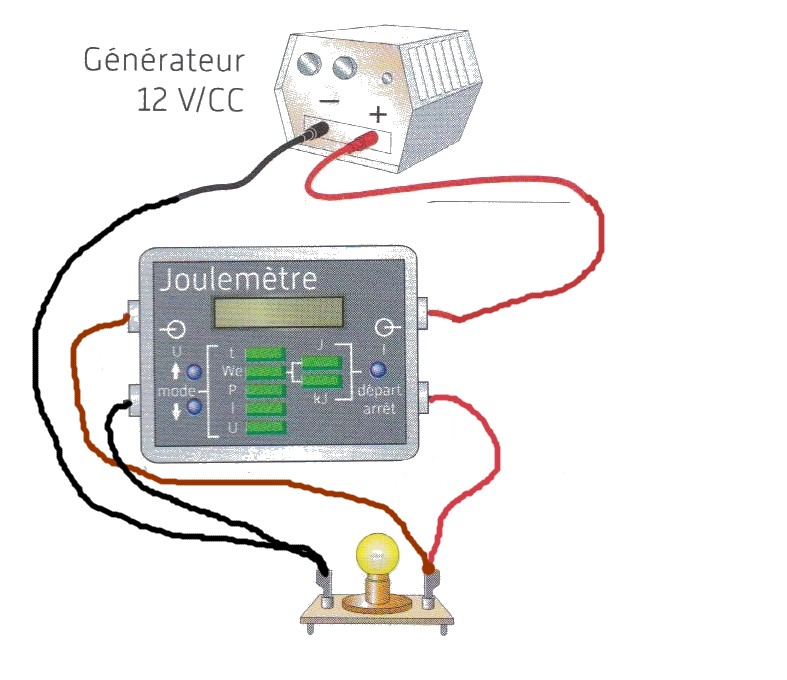
\includegraphics[width=\textwidth]{images/TP1 - Montage.jpg}\end{center}
\end{minipage}%

\vfill 

\fcolorbox{black}{blue!30}{\textbf{Protocole}}
\begin{itemize}
    \item Réaliser le montage électriques ci-dessus.
    
\defbox{\fbox{
\begin{minipage}{10cm}{

Appeler M Ruiz pour qu'il vérifie le montage. $\Box \Box \Box ~~\raisebox{0.3ex}{\bigcirc}$}

\end{minipage}
}} 

    \item Réglez le joule mètre en mode puissance et relevez la valeur de la puissance $P$ reçue par la lampe allumée. 
    \begin{center}
        \vspace{-5mm} 
        \fbox{\Large{P = .......} }
    \end{center}
    \item Réglez le joulemètre en mode énergie et relevez la valeur de l'énergie $E$ reçue par la lampe allumée pour des durées $t$ égales à 60s, 120s, 180s et 240s. \\ Noter les valeurs dans le tableau ci-dessous. 
\end{itemize}

\begin{center}
    

    \begin{tabular}{|C{2cm}||C{2cm}|C{2cm}|C{2cm}|C{2cm}|}
         \hline
         Durée $t$ (s)& 60 & 120 & 180 & 240\\
         \hline
         Énergie (J)&  &  &  & \\
         \hline
    \end{tabular}
\end{center}

\vfill

\fcolorbox{black}{blue!30}{\textbf{Mesures}}\\
\ding{202} Complétez le tableau suivant à l'aide de vos mesures : 

\begin{center}
    

    \begin{tabular}{|C{2cm}||C{2cm}|C{2cm}|C{2cm}|C{2cm}|}
         \hline
                  P (W) &  &  &  & \\
         \hline
         Durée $t$ (s)& 60 & 120 & 180 & 240\\
         \hline

         $P \times t$ &  &  &  & \\
         \hline
         Énergie (J)&  &  &  & \\
         \hline
    \end{tabular}
\end{center}
\vfill 

\newpage

\ding{203} Tracez la représentation graphique modélisant l'énergie mesurée $E$ en $J$ en fonction du temps $t$ en $s$
\begin{center}
    




\begin{tikzpicture}[scale=1]
%papier milli
\draw [very thin, gray!20] (0,-3) grid[step=0.1] (13,6);

\draw [very thin, black!20] (0,-3) grid[step=0.5] (13,6);
\draw [very thin, black!40] (0,-3) grid[step=1] (13,6);
\draw[->,>=stealth] (0,-3) -- (13.5,-3) node[below right] {t(ms)};
%stealth définit un style de flèche, "furtif"
\draw[->,>=stealth] (0,-3) -- (0,6.2)node[below left] {E(J)};

\draw (0,-2.9) -- (0,-3.1) node [below left] {{\scriptsize 0}}; 
\draw (3,-2.9) -- (3,-3.1) node [below left] {{\scriptsize 60}}; %échelle abscisse
\draw (0.1,-1) -- (-0.1,-1) node [left] {{\scriptsize 
1000}}; %échelle ordonnée

\end{tikzpicture}
\end{center}

\vfill 

\fcolorbox{black}{blue!30}{\textbf{Interprétation }} \\[5mm]
\ding{204} Commentez la représentation graphique que vous avez obtenue. \\
\cadreblanc{25}
\ding{205} Comparez le produit $P \times t$ à $E$ reçue par la lampe \\
\cadreblanc{10}
\ding{206} Que peut-t-on dire de $E$ par rapport à $t$ \\
\cadreblanc{10}



\vfill
\fcolorbox{black}{blue!30}{\textbf{Conclusion}}\\[5mm]
\ding{207}  Écrivez la formule liant $E$, $P$ et $t$ en précisant les unités de ces trois grandeurs. 
\begin{center}
   \begin{minipage}{5cm}
   \cadreblanc{20}
   \end{minipage}
\end{center}

\vfill 


\end{document}